%!TEX TS-program = xelatex

\documentclass[10pt]{article}

\usepackage[usenames,dvipsnames,svgnames,table,xcdraw]{xcolor}

%%%%% LANGUAGE AND FONTS 
\usepackage{xltxtra,xgreek,fontspec}
\usepackage[T1]{fontenc}
\setmainfont{Times New Roman} 			 % main font
\setmonofont{Courier New}			 	 % for commands
\usepackage[greek]{datetime2} 		 % show greek date correctly using \today command
\renewcommand{\today}{\ifcase\month\or%
Ιανουάριος\or Φεβρουάριος\or Μάρτιος\or% 
Απρίλιος\or Μάιος\or Ιούνιος\or Ιούλιος%
\or Αύγουστος\or Σεπτέμβριος\or% 
Οκτώβριος\or Νοέμβριος\or% 
Δεκέμβριος\fi\ \number \year}			 % nominative instead of genitive 
\usepackage{amsmath}

%%%%% SPACING AND GEOMETRY
\usepackage[textwidth=17cm,
textheight=23cm]{geometry} 							% document geometry
\addtolength{\voffset}{0.5cm}						% vertical space between top of page and bottom of header
\usepackage{setspace}							% set space between lines
\usepackage[flushmargin, hang, bottom]{footmisc}% optimize footer spacing
\addtolength{\footnotesep}{2.5mm}					% space between footnotes
\usepackage{float} 								% provides H option for precise position of figure environments
\usepackage{array} 								% extra option for arrays and columns format ( like m{} ) 
\newcommand{\dnormalspacing}{1.25}					% line spacing
\renewcommand{\baselinestretch}{\dnormalspacing}    % set line streching
\usepackage{titlesec}							% customize space and place of section, subsection	
\setlength{\parindent}{0pt}							% no horizontal space on new paragraph
\setlength{\parskip}{1em}							% space between each paragraph
\titlespacing{\section}{0pt}{0pt}{0pt}				% [default] no extra space between section 
\titlespacing{\subsection}{0pt}{0pt}{0pt}			% [default] no extra space between subsection
\AtBeginEnvironment{itemize}{\vspace*{-0.3cm}}
\AtBeginEnvironment{enumerate}{\vspace*{-0.3cm}}
\usepackage{multirow}
\usepackage{enumitem}
\setlist{itemsep=1pt}

%%%%% BOXES AND LAYOUTS
\usepackage{changepage}  % page layout customization
\usepackage{booktabs}	 % extra commands for tables like \cmidrule{}
\usepackage{tabularx}
\usepackage{fancyhdr}	 % customize footer and header layouts
\pagestyle{fancy}														
\fancyhf{}	
\lhead{\footnotesize Κλάση EdipyLabs.sty}									 						
\rhead{\footnotesize Εργαστήριο Δικτύων και Προηγμένων Υπηρεσιών}	% COURSE title, change it if you want to
\cfoot{\noindent\makebox[\linewidth]{\rule{0.75cm}{0.4pt}}\\\thepage} % custom page number format
\usepackage[framemethod=tikz]{mdframed}


%%%%% COLOURS, GRAPHICS AND FIGURES
\usepackage{graphicx} 					% more options for \includegraphics
\usepackage{soulutf8}				% soul provides \hl for highlighting text
\usepackage[font={small,singlespacing},
labelfont={bf},
textfont={it},
justification={justified},
margin=0pt]{caption}						% customization of captions on figures 
\usepackage{hyperref} 					% hyperlink customization
\usepackage{tikz}						% used to create \keystroke command
\usetikzlibrary{shadows}
\graphicspath{{./figures/}}  				% All imported figures must be in a folder named 'figures'

\usepackage{titling}

\pretitle{\begin{center}\Huge\bfseries}
	\posttitle{\par\end{center}\vskip 0.5em}
\preauthor{\begin{center}\Large\ttfamily}
	\postauthor{\end{center}}
\predate{\par\large\centering}
\postdate{\par}

\title{Η κλάση EdipyLabs.cls}
\author{Χρήστος Δαλαμάγκας\\ <cdalamagkas@gmail.com>}
\date{\today}

\begin{document}
	
\maketitle
\thispagestyle{empty}

\begin{abstract}
	H κλάση \texttt{EdipyLabs.sty} αναπτύχθηκε για την συγγραφή εργαστηριακών φυλλαδίων, ειδικά για το Εργαστήριο Δικτύων και Προηγμένων Υπηρεσιών του Τμήματος Μηχανικών Πληροφορικής και Τηλεπικοινωνιών, του Πανεπιστημίου Δυτικής Μακεδονίας. Η κλάση υποστηρίζει πλήρως την ελληνική γλώσσα και απαιτεί τον οδηγό XeLaTeX για τη μεταγλώττιση. 
\end{abstract}
\tableofcontents
	 
\section{Οδηγίες εγκατάστασης}
Το αρχείο \texttt{EdipyLabs.sty} και το λογότυπο του Πανεπιστημίου πρέπει να βρίσκονται είτε στον ίδιο φάκελο με τον πηγαίο κώδικα \texttt{.tex} του εργαστηριακού φυλλαδίου που προετοιμάζετε ή σε έναν κατάλογο ρίζας TEXMF. Αν χρησιμοποιείτε το MikTex, οι προεπιλεγμένοι κατάλογοι ρίζας TEXMF παρατίθενται στον εξής ιστότοπο: \url{https://miktex.org/kb/texmf-roots}.

Εκτός από τους προεπιλεγμένους καταλόγους, μπορείτε να ορίσετε και έναν δικό σας φάκελο ως κατάλογο ρίζας TEXMF. Στα συστήματα Windows και για τη διανομή MikTeX, μπορείτε να προσθέσετε έναν φάκελο ως ρίζα στο παράθυρο MikTex Settings (Admin), όπως φαίνεται στην παρακάτω εικόνα:

\begin{figure}[ht]
 	\centering
 	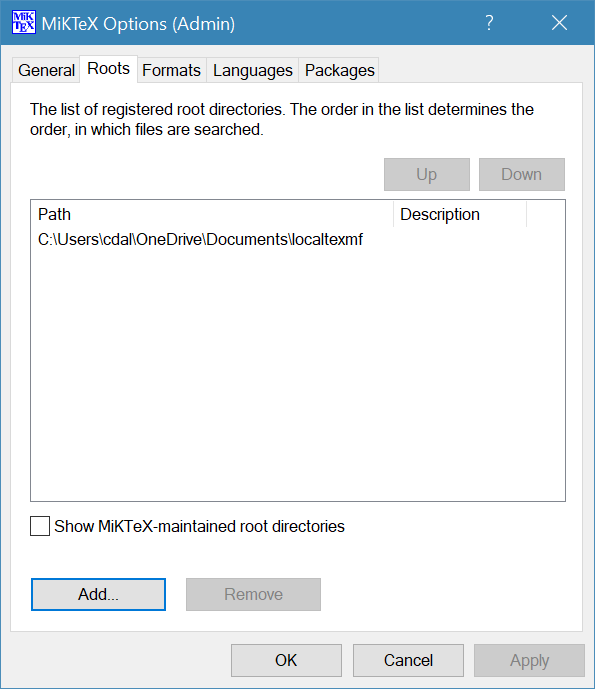
\includegraphics[width=0.35\linewidth]{texmfroot.PNG}
\end{figure}
	 
Ένας κατάλογος ρίζας TEXMF πρέπει κατ' ελάχιστον να περιέχει έναν φάκελο με το όνομα \texttt{tex} και, μέσα σε αυτόν, έναν υποφάκελο με όνομα \texttt{latex}. Όλες οι πρόσθετες κλάσεις και τα πακέτα που δεν έχουν εγκατασταθεί αυτόματα από τη διανομή LaTeX μπορούν να προστεθούν στον υποφάκελο \texttt{latex}. 



\section{Επιλογές κλάσης}

\section{Οδηγός εκκίνησης}

\section{Παραμετροποιήσεις της κλάσης}

\section{Νέες εντολές}
	
\end{document}

